\documentclass{article}
\usepackage{graphicx}
\usepackage{hyperref}

\title{\textbf{Exploring the use of LLMs for Web Scraping}}
\author{
	João Cardoso, No. 50465, \texttt{a50465@alunos.isel.pt}, tel.: 933840873 \\
	\and
	Francisco Antunes, No. 50497, \texttt{a50497@alunos.isel.pt}, tel.: 962225712 \\
	\and
	Rúben Said, No. 47526, \texttt{a47526@alunos.isel.pt}, tel.: 963756360
	\and
	\\
	 Supervisor: Paulo Pereira, e-mail: paulo.pereira@isel.pt
}
\begin{document}
	\begin{figure}[htbp]
		\begin{center}
			\includegraphics[scale=0.4]{/home/cardosodev04/Documents/Faculdade/PFC/PFC - GenAI/Proposta/proposta-latex/imgs/logo_ISEL_principal_PNG.png}	
			\maketitle
		\end{center}
	\end{figure}
	\pagebreak
	\section{Introduction}
	\setlength\parindent{24pt}
	Companies such as Tryp.com face significant challenges related to semantic changes on third-party websites during the process of automating actions on these platforms.
	
	Traditionally, this process is achieved through the implementation of a technique known as web scraping. However, this technique, as currently employed, proves to be fragile and particularly prone to errors, primarily due to the dynamic nature of web pages.
	
	In light of this scenario, this project proposes exploring the use of Large Language Models (LLMs) and Generative Artificial Intelligence as decision-making mechanisms. The aim is to develop an adaptive solution that enhances the robustness of the web scraping process and the formulation of automated actions. These actions will be executed by a software agent designed to operate in place of a human user.
	\pagebreak
	
	\section{Technical Requirements}
	\subsection{Functional Requirements}
		We should create an AI agent capable of extracting HTML from a webpage (statically or dynamically generated) and analyzing it in order to identify possible actions and execute them in a chain when given a final goal.
        
		The agent's decision mechanism should be based on a locally deployed large language model (LLM).
        
		The agent should first be able to identify and generate a representation, in a normalized manner, of the possible interactions it can have with the webpage.
		Given the normalized format mentioned above, the agent should be able to formalize a chain of currently available actions when given a final goal.
        
		The agent should be able to evaluate, after each interaction, whether the end goal has been achieved. If not, it should generate a new representation upon the completion of the said action so that it can continue executing. 
	\subsection{Non-Functional Requirements}
		The agent's user should be able to interact with it through an intuitive GUI.
        
		The agent should demonstrate high reliability, capable of handling web pages of medium to high complexity with minimal failure occurrences. It should gracefully handle unexpected changes in webpage structure or content.
        
		This project should follow Clean Architecture principles ensuring it's maintainability, readability and eventual scalability.
        
		The software produced for this project should be thoroughly tested and validated at each step of the way.
	\subsection{Optional features}
	\begin{itemize}
		\item An automatically generated visual representation of the current chain of actions in a locally served webpage.
		\item Test reports exposing each step taken by the agent and the final result.
	\end{itemize}
	
	\pagebreak
	
	\section{Technologies}
	\setlength\parindent{24pt}		
        We plan to develop this project using \textbf{Kotlin} with \textbf{Gradle}, adopting a modular and extensible architecture. The backend will integrate with a locally deployed \textbf{Large Language Model} (LLM) via the \textbf{Ollama} Web API served locally by the Ollama application, ensuring efficient and scalable interaction. Additionally, the automation and data extraction process will be conducted using Selenium, a framework traditionally employed for web application testing.
	\begin{figure}[htbp]
	\centering
	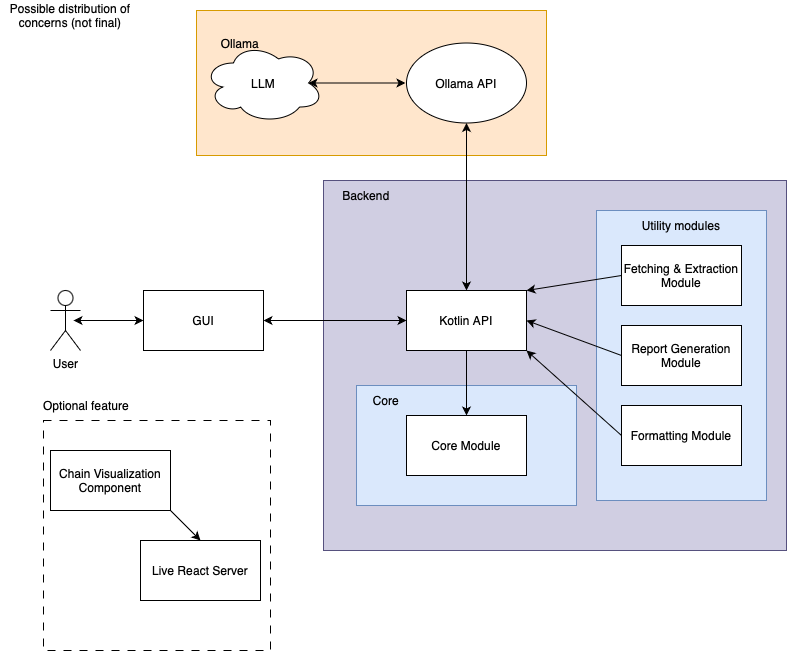
\includegraphics[scale=0.4]{PFC - V2.drawio.png}	
	\caption{Software organization diagram}
	\end{figure}
	
	\section{Risks and challenges}
	\begin{itemize}
		\item We have never worked with LLMs, AI or prompt engineering before, so that could pose a challenge as we will have to learn new technologies.
		\item LLMs are known to be inconsistent and hallucinate; this is a considerable risk since we want our agent to be as reliable as possible.
	\end{itemize}
	
	\section{Project timeline}
	
	\pagebreak
	
		\begin{thebibliography}{9}
			\bibitem{cloudflare} 
			Cloudflare - What is a Large Language Model? - \texttt{https://www.cloudflare.com/learning/ai/what-is-large-language-model/}
			
			\bibitem{ollama} 
			Ollama's official website - \texttt{https://ollama.com/}
		\end{thebibliography}
	
\end{document}

